\documentclass[tikz,border=5pt]{standalone}
\usepackage{luatexja}
\usepackage[hiragino-pron]{luatexja-preset}
\usepackage{amsmath,amssymb}
\usepackage{pgfplots}
\pgfplotsset{compat=1.18}
\usetikzlibrary{arrows.meta,calc,decorations.markings,patterns,positioning}

% Common styles
\tikzset{
  axis/.style={-{Stealth[length=6pt]}, thick},
  curve/.style={thick, red},
  dashed curve/.style={thick, dashed, blue},
  dot/.style={circle, fill, inner sep=1.5pt},
  open dot/.style={circle, draw, fill=white, inner sep=1.5pt},
}

\begin{document}
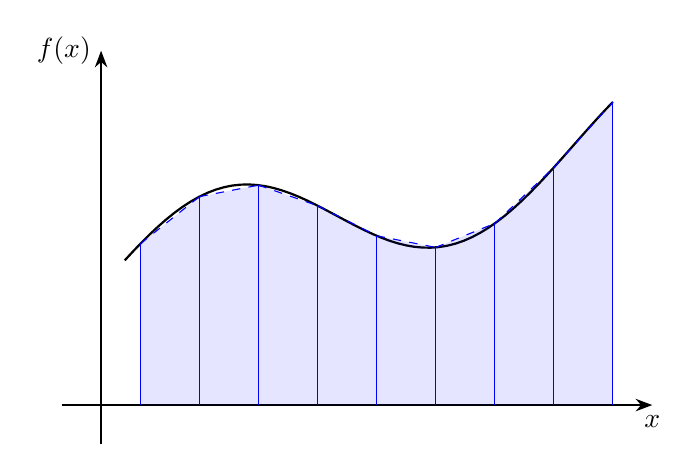
\begin{tikzpicture}
  % Axes
  \draw[axis] (-0.5,0) -- (7,0) node[below] {$x$};
  \draw[axis] (0,-0.5) -- (0,4.5) node[left] {$f(x)$};

  % Smooth curve
  \draw[thick, domain=0.3:6.5, samples=60]
    plot (\x, {1.5 + 0.8*sin(60*\x) + 0.3*\x});

  % Piecewise linear approximation (rectangles)
  \foreach \i in {0,...,7} {
    \pgfmathsetmacro{\xl}{0.5 + 0.75*\i}
    \pgfmathsetmacro{\xr}{0.5 + 0.75*(\i+1)}
    \pgfmathsetmacro{\xm}{0.5*(\xl+\xr)}
    \pgfmathsetmacro{\yl}{1.5 + 0.8*sin(60*\xl) + 0.3*\xl}
    \pgfmathsetmacro{\yr}{1.5 + 0.8*sin(60*\xr) + 0.3*\xr}
    % Rectangle (trapezoid approximation)
    \draw[blue, thin] (\xl,0) -- (\xl,\yl);
    \draw[blue, thin] (\xr,0) -- (\xr,\yr);
    \draw[blue, dashed, thin] (\xl,\yl) -- (\xr,\yr);
    % Fill
    \fill[blue, opacity=0.1] (\xl,0) -- (\xl,\yl) -- (\xr,\yr) -- (\xr,0) -- cycle;
  }
\end{tikzpicture}
\end{document}
